%%%%%%%%%%%%%%%%%%%%%%%%%%%%%%%%%%%%%%%%%%%%%%%%%%%%%%%%%%%%%%%%%%%%%%%%%%%%%%%
%
% Evaluation
% 
%%%%%%%%%%%%%%%%%%%%%%%%%%%%%%%%%%%%%%%%%%%%%%%%%%%%%%%%%%%%%%%%%%%%%%%%%%%%%%%


\chapter{Results}
\label{sec:results}

\section{Results}

\newpage

\begin{figure}[H]
\centering
\subfloat[1]{
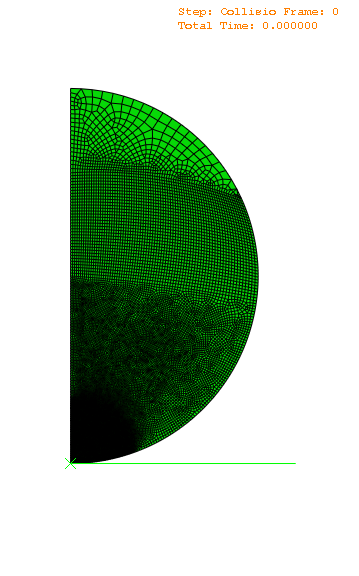
\includegraphics[width=0.20\textwidth]{../images/motion/1.png}
\label{fig:motion1}
}
\subfloat[2]{
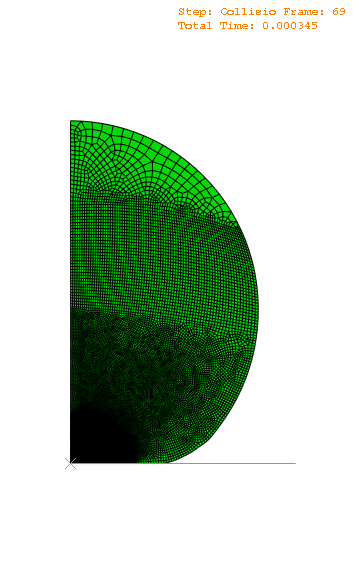
\includegraphics[width=0.20\textwidth]{../images/motion/2.png}
\label{fig:motion2}
}
\subfloat[3]{
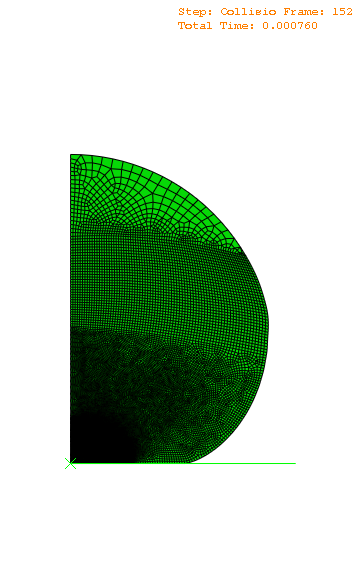
\includegraphics[width=0.20\textwidth]{../images/motion/3.png}
\label{fig:motion3}
}
\subfloat[4]{
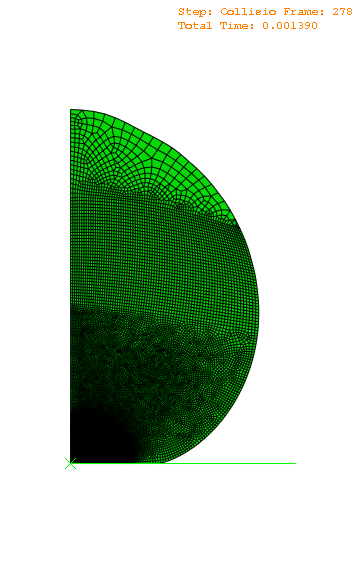
\includegraphics[width=0.20\textwidth]{../images/motion/4.png}
\label{fig:motion4}
}

\subfloat[5]{
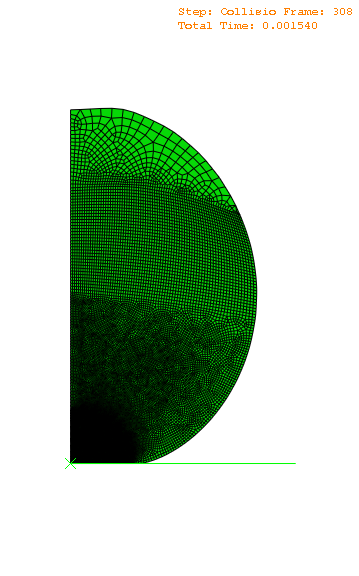
\includegraphics[width=0.20\textwidth]{../images/motion/5.png}
\label{fig:motion5}
}
\subfloat[6]{
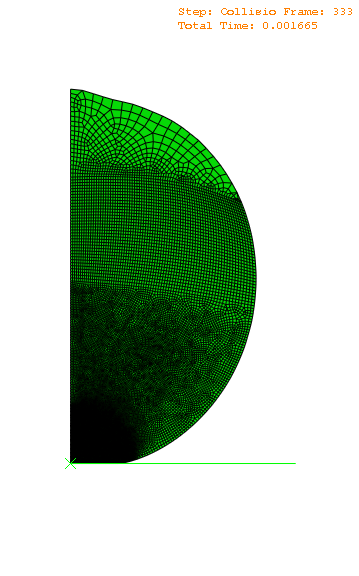
\includegraphics[width=0.20\textwidth]{../images/motion/6.png}
\label{fig:motion6}
}
\subfloat[7]{
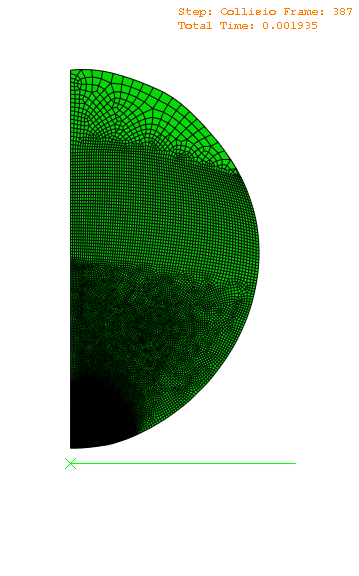
\includegraphics[width=0.20\textwidth]{../images/motion/7.png}
\label{fig:motion7}
}
\subfloat[8]{
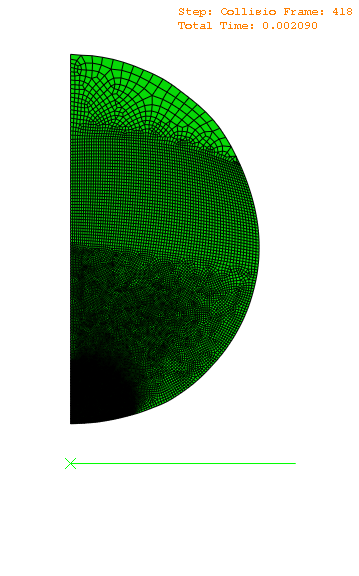
\includegraphics[width=0.20\textwidth]{../images/motion/8.png}
\label{fig:motion8}
}

\subfloat[9]{
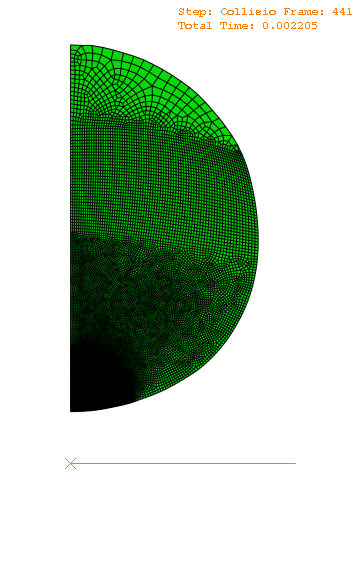
\includegraphics[width=0.20\textwidth]{../images/motion/9.png}
\label{fig:motion9}
}
\subfloat[10]{
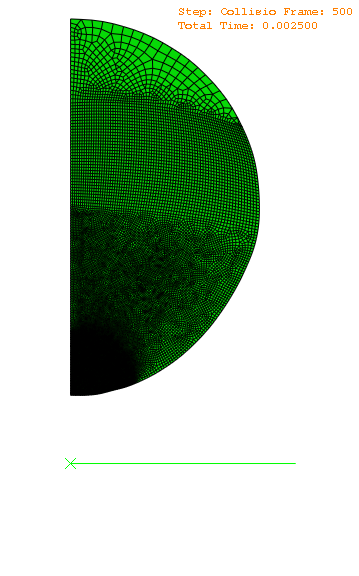
\includegraphics[width=0.20\textwidth]{../images/motion/10.png}
\label{fig:motion10}
}
\caption{A very soft material\label{fig:motion}}
\end{figure}

As we study the loss of kinetic energy to vibrations let's first consider a very soft material. The series of figures in \ref{fig:motion} shows the trajectory of a very soft material with Young Modulus($E$)$ = 6 MPa$ with an impact velocity of $5m/s$. After the contact is lost, spheres starts to vibrate violently. This shows that some part of the kinetic energy possessed by the sphere is converted to strain energy which then caused the vibrations in the sphere. 


%%%%%%%%%%%%%%%%%Force%%%%%%%%%%%%%%%%
\subsection{Contact Force}

\begin{figure}[!htbp]
\centering
\subfloat[Velocity 0.01m/s]{
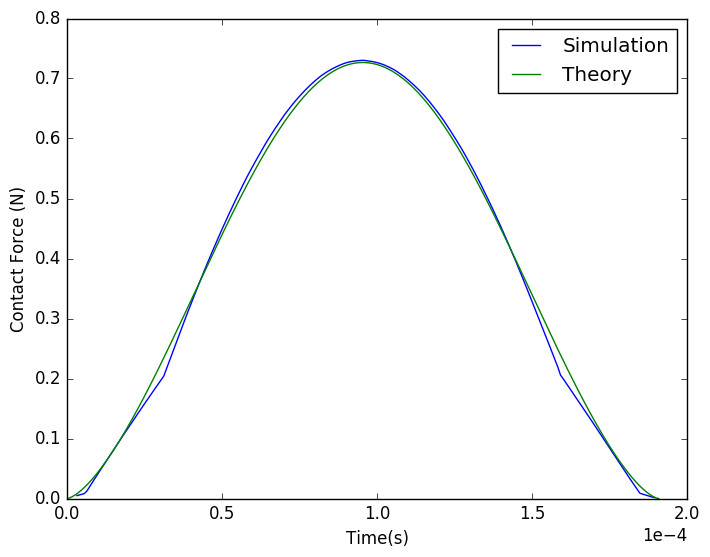
\includegraphics[width=0.50\textwidth]{{../images/force/Force-vel1.0}.png}
\label{fig:force1}
}
\subfloat[Velocity 0.10m/s]{
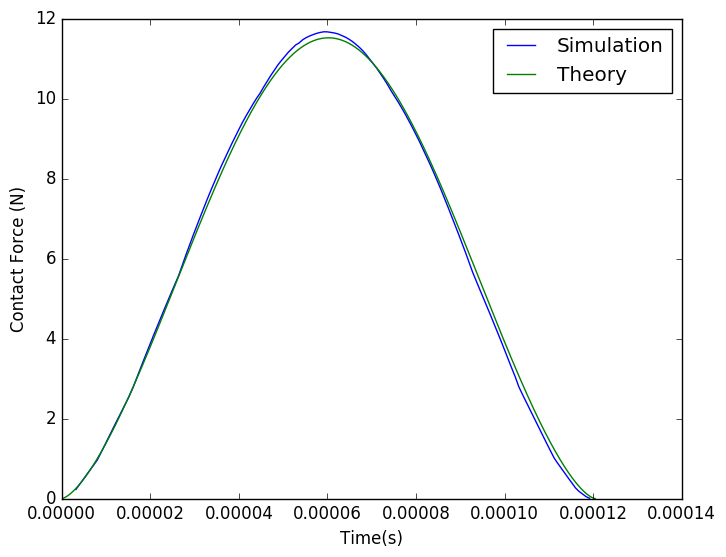
\includegraphics[width=0.50\textwidth]{{../images/force/Force-vel10.0}.png}
\label{fig:force10}
}

\subfloat[Velocity 0.20m/s]{
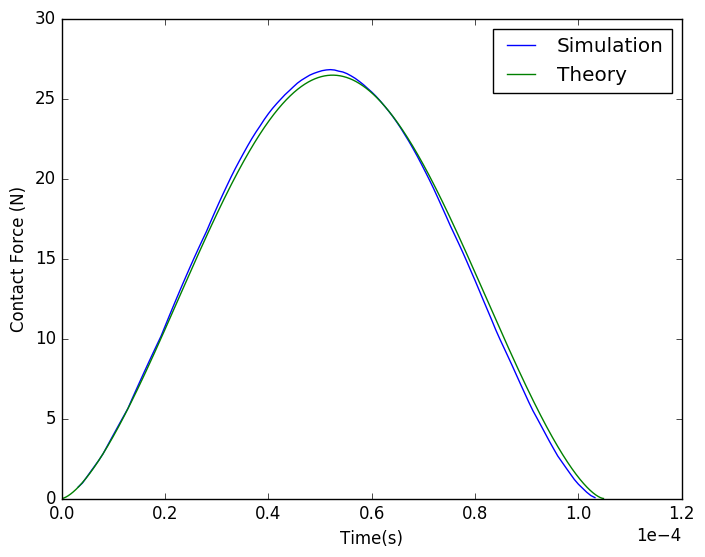
\includegraphics[width=0.50\textwidth]{{../images/force/Force-vel20.0}.png}
\label{fig:force20}
}
\subfloat[Velocity 0.30m/s]{
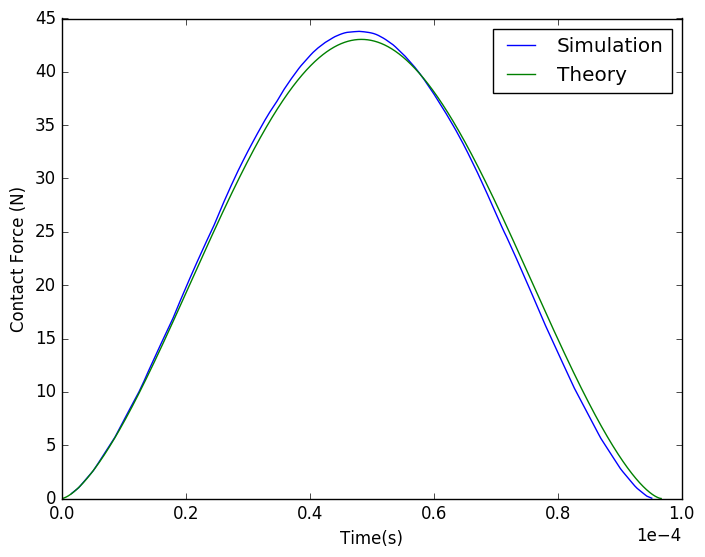
\includegraphics[width=0.50\textwidth]{{../images/force/Force-vel30.0}.png}
\label{fig:force30}
}

\subfloat[Velocity 1.0m/s]{
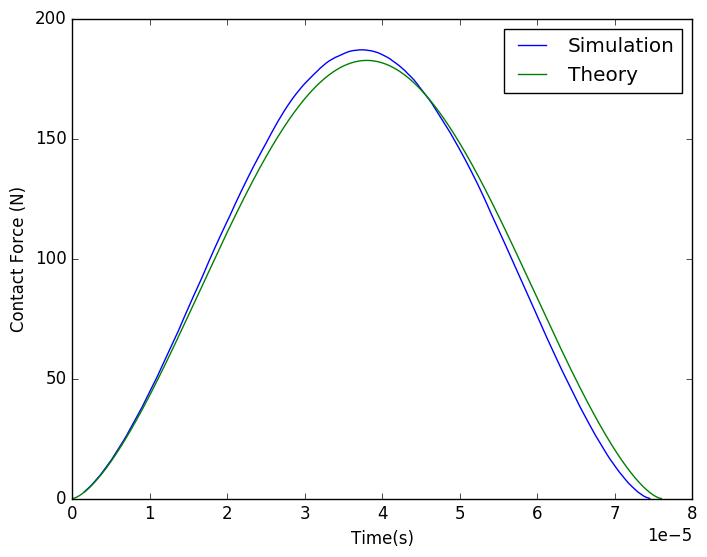
\includegraphics[width=0.50\textwidth]{{../images/force/Force-vel100.0}.png}
\label{fig:force50}
}
\subfloat[Velocity 3.0m/s]{
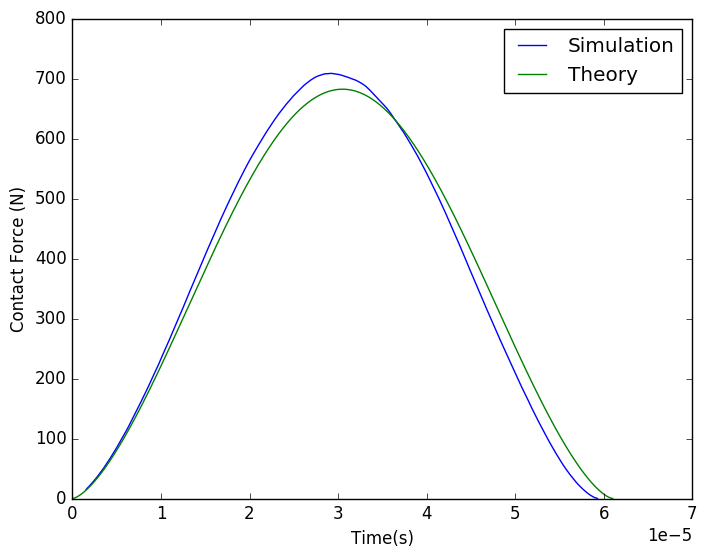
\includegraphics[width=0.50\textwidth]{{../images/force/Force-vel300.0}.png}
\label{fig:force300}
}
\caption{Contact force vs Time for various impact velocities}
\label{fig:force}
\end{figure}

Now considering a harder material, i.e. with $Youngs Modulus(E)$ of $9.3GPa$. This Youngs Modulus was chosen as it was neither to hard nor to soft and had the vibration visible. The plots in \ref{fig:def} show the contact force between the sphere and the rigid plane. The plots shows that as the impact velocities are higher, the difference between the simulation data and the theoretical data is more visible. This errors is due the quasi static assumptions.


%%%%%%%%%%%%%%%%%%COM%%%%%%%%%%%%%%%%%%%

\subsection{Deformation}

\begin{figure}[!htbp]
\centering
\subfloat[Velocity 0.01m/s]{
\includegraphics[width=0.50\textwidth]{{../images/deformationVStime/Velocity1.0}.png}
\label{fig:def1}
}
\subfloat[Velocity 0.10m/s]{
\includegraphics[width=0.50\textwidth]{{../images/deformationVStime/Velocity10.0}.png}
\label{fig:def10}
}

\subfloat[Velocity 0.20m/s]{
\includegraphics[width=0.50\textwidth]{{../images/deformationVStime/Velocity20.0}.png}
\label{fig:def20}
}
\subfloat[Velocity 0.30m/s]{
\includegraphics[width=0.50\textwidth]{{../images/deformationVStime/Velocity30.0}.png}
\label{fig:def30}
}

\subfloat[Velocity 1m/s]{
\includegraphics[width=0.50\textwidth]{{../images/deformationVStime/Velocity100.0}.png}
\label{fig:def50}
}
\subfloat[Velocity 3.0m/s]{
\includegraphics[width=0.50\textwidth]{{../images/deformationVStime/Velocity300.0}.png}
\label{fig:def300}
}
\caption{Displacement of the center of the sphere for various impact velocities}
\label{fig:def}
\end{figure}

The plots in \ref{fig:def} show displacement of the center point of the sphere with respect to time. The plots shows that as the impact velocities are higher, the difference between the simulation data and the theoretical data is more visible. This errors is due the quasi static assumptions. But unfortunately these plot are not conclusive as the velocity of the center of mass is the velocity which should be compared and not the velocity of the center of the sphere.


%%%%%%%%%%%%%%%%%%Energy%%%%%%%%%%%%%%%%%%%%


\subsection{Energy}
\begin{figure}[H]
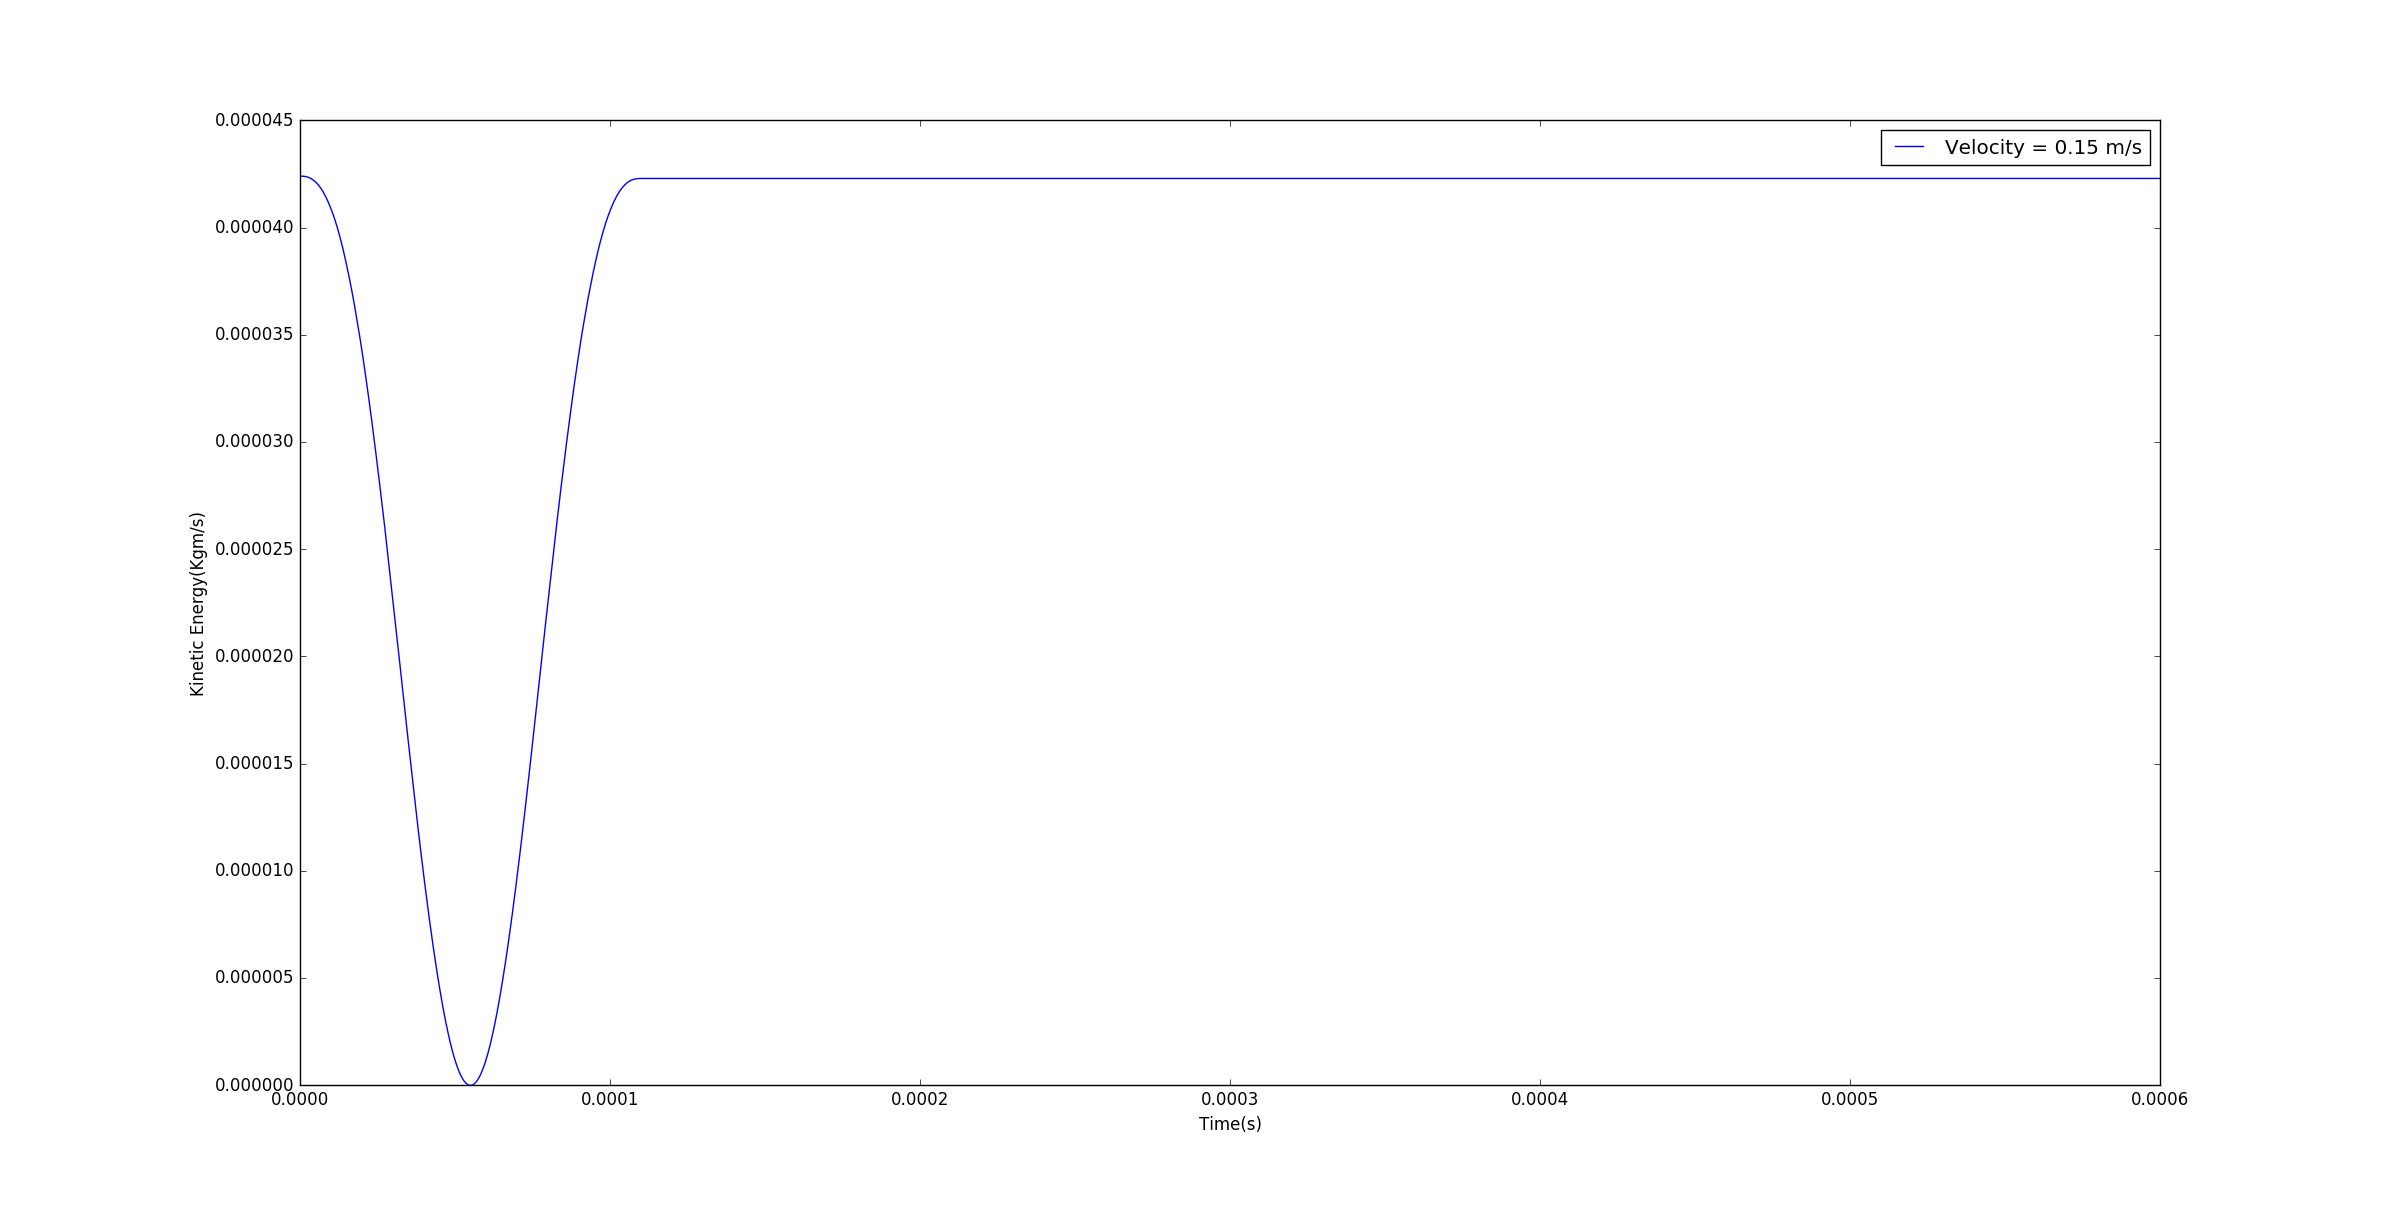
\includegraphics[width=1.0\textwidth]{../images/KE/KE.png}
\caption{Kinetic Energy}
\label{fig:KE}
\end{figure}
\begin{figure}[H]
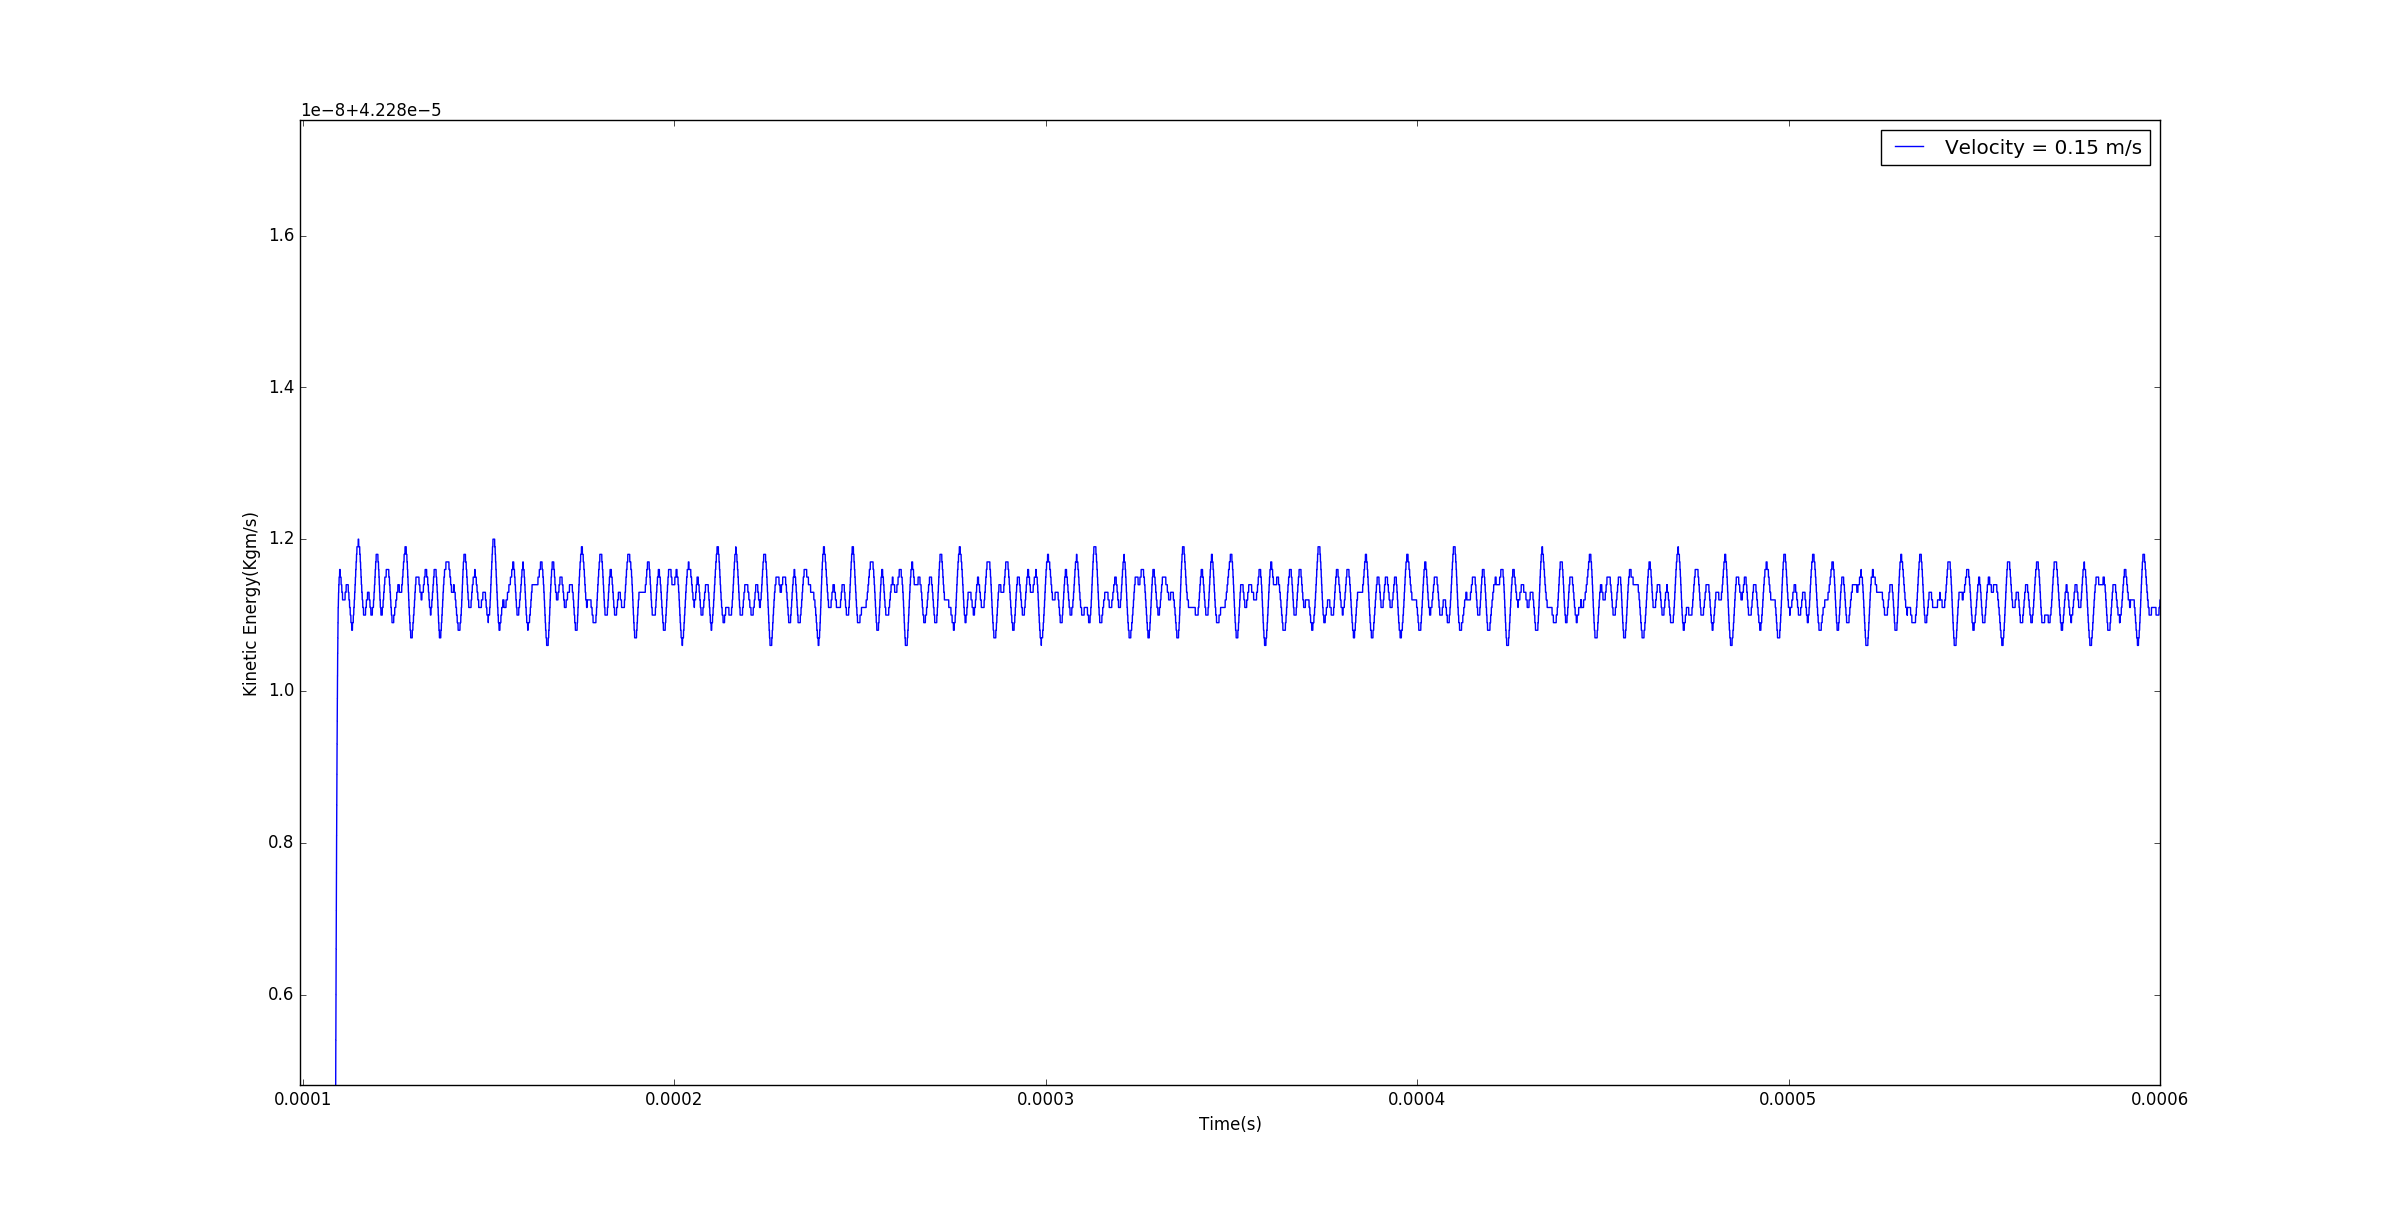
\includegraphics[width=1.0\textwidth]{../images/KE/KE-zoomed.png}
\caption{Kinetic Energy contact is broken}
\label{fig:KEzoomed}
\end{figure}
The figure \ref{fig:KE} shows Kinetic Energy vs Time for the impact velocity of $0.15m/s$. It is clear that the kinetic energy decreases in the beginning of the impact and increases towards the end of the impact. When observed carefully, fluctuations can be observed in the plot after the impact is completed as shows in \ref{fig:KEzoomed}. As disscussed in the previous paragraphs, this is because a part of the kinetic energy is converted into strain energy which cause vibrations in within the model.

A similar trend is also visible in the plot of the strain energy of the sphere. It is clear from \ref{fig:SEzoomed}, that after the collision is complete, the body still possesses a small amount of strain energy.

\begin{figure}[H]
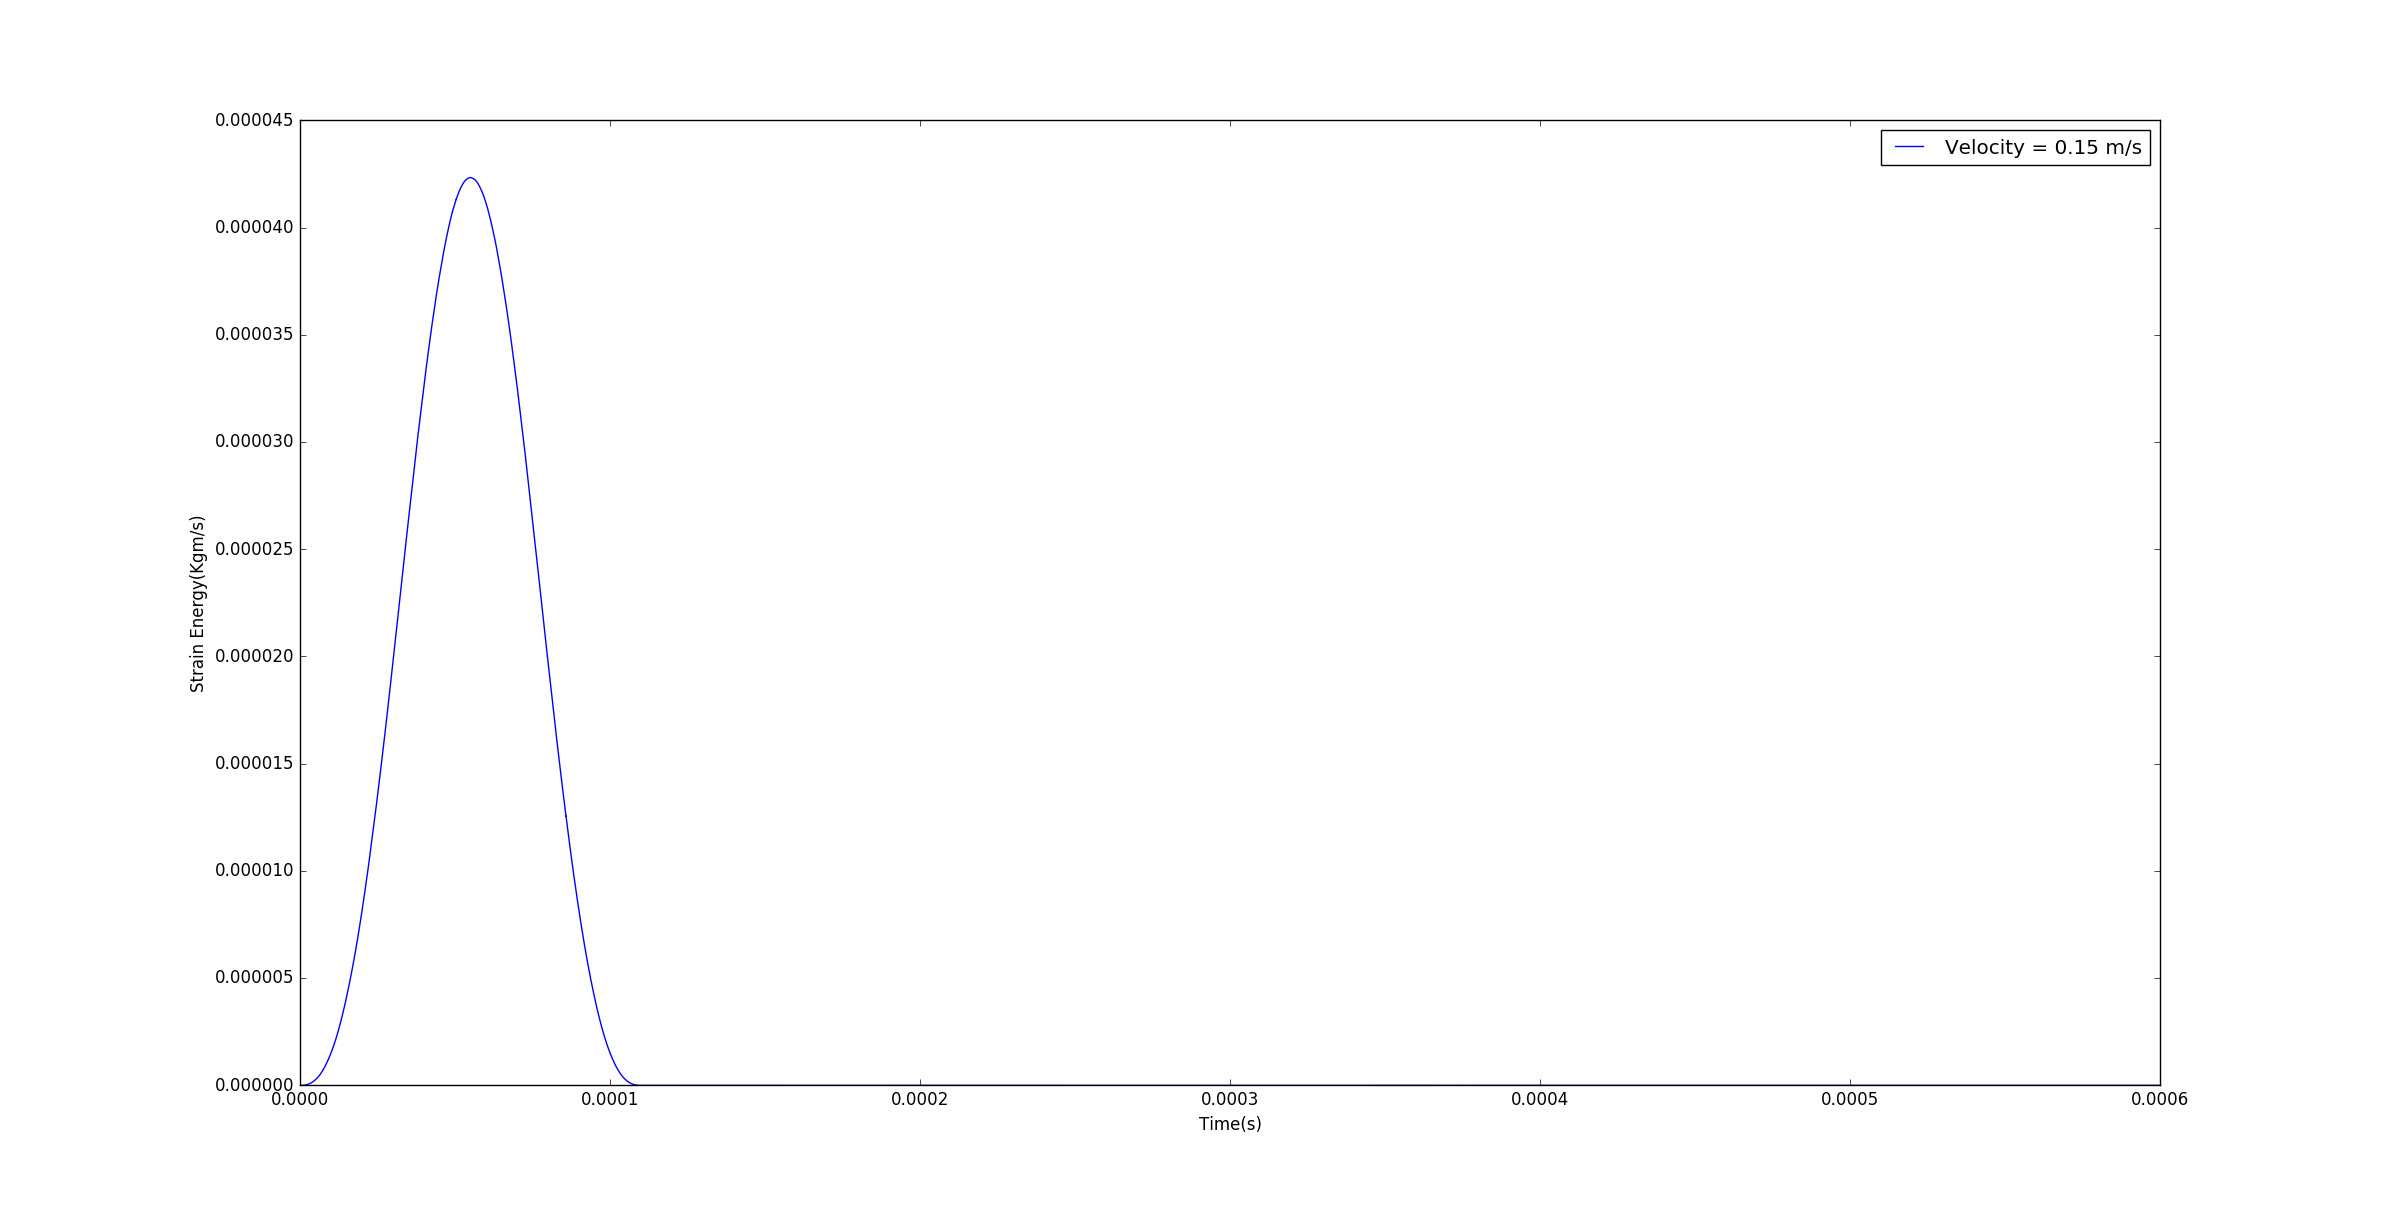
\includegraphics[width=1.0\textwidth]{../images/StrainEnergy/strainenergy.png}
\caption{Strain Energy}
\label{fig:SE}
\end{figure}
\begin{figure}[H]
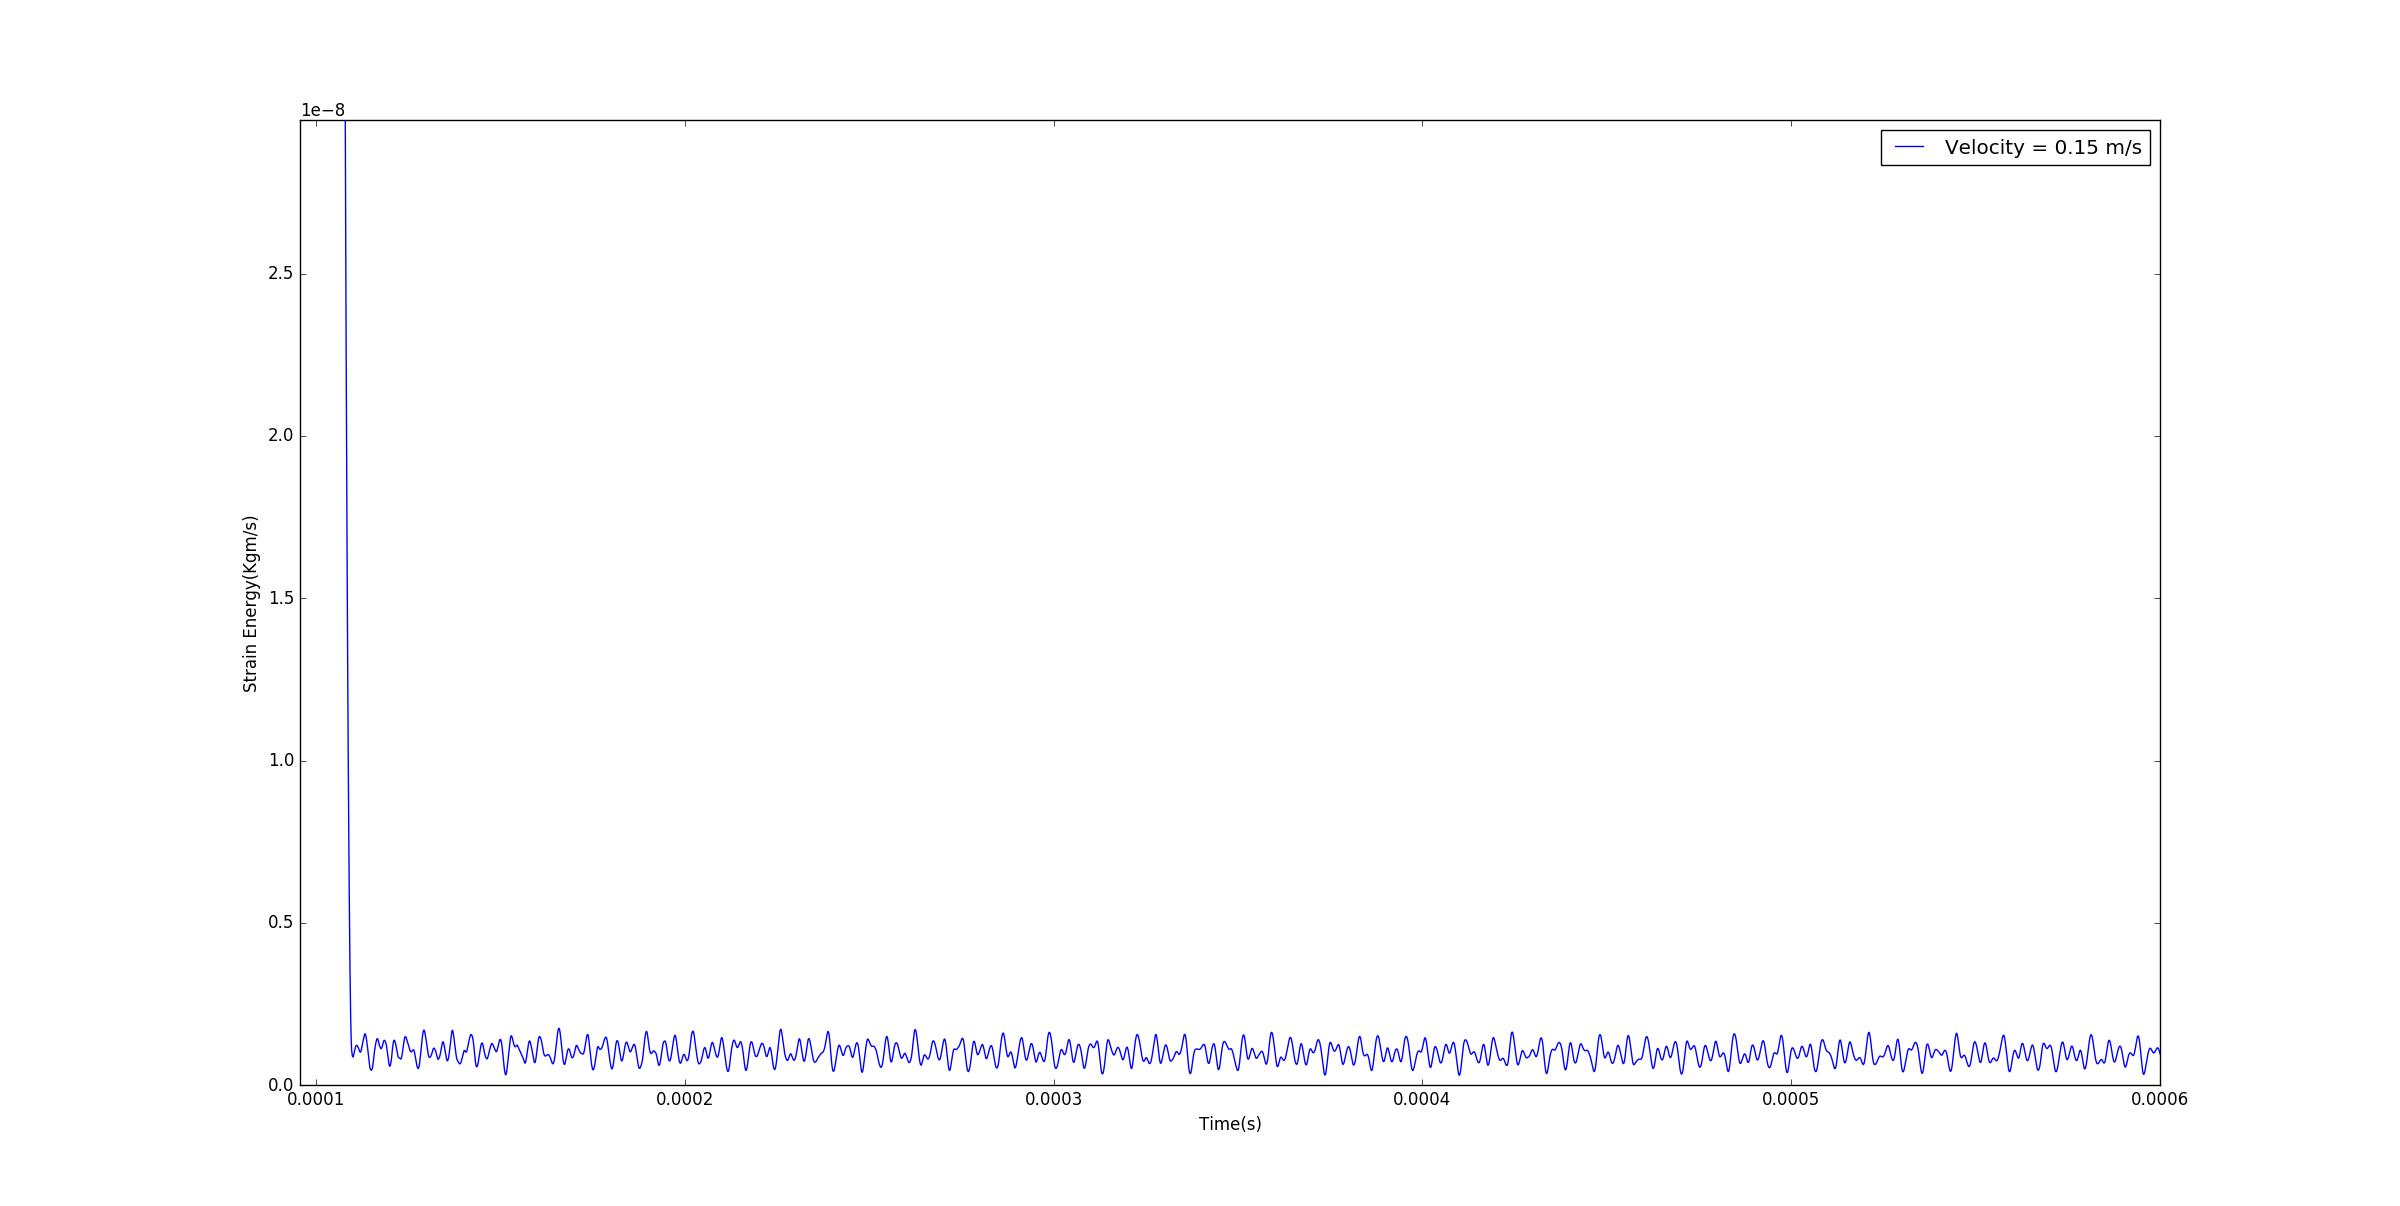
\includegraphics[width=1.0\textwidth]{../images/StrainEnergy/strainenergy-zoomed.png}
\caption{Strain Energy after contact is broken}
\label{fig:SEzoomed}
\end{figure}


\subsection{Co-efficient of Restitution}

\begin{figure}[H]
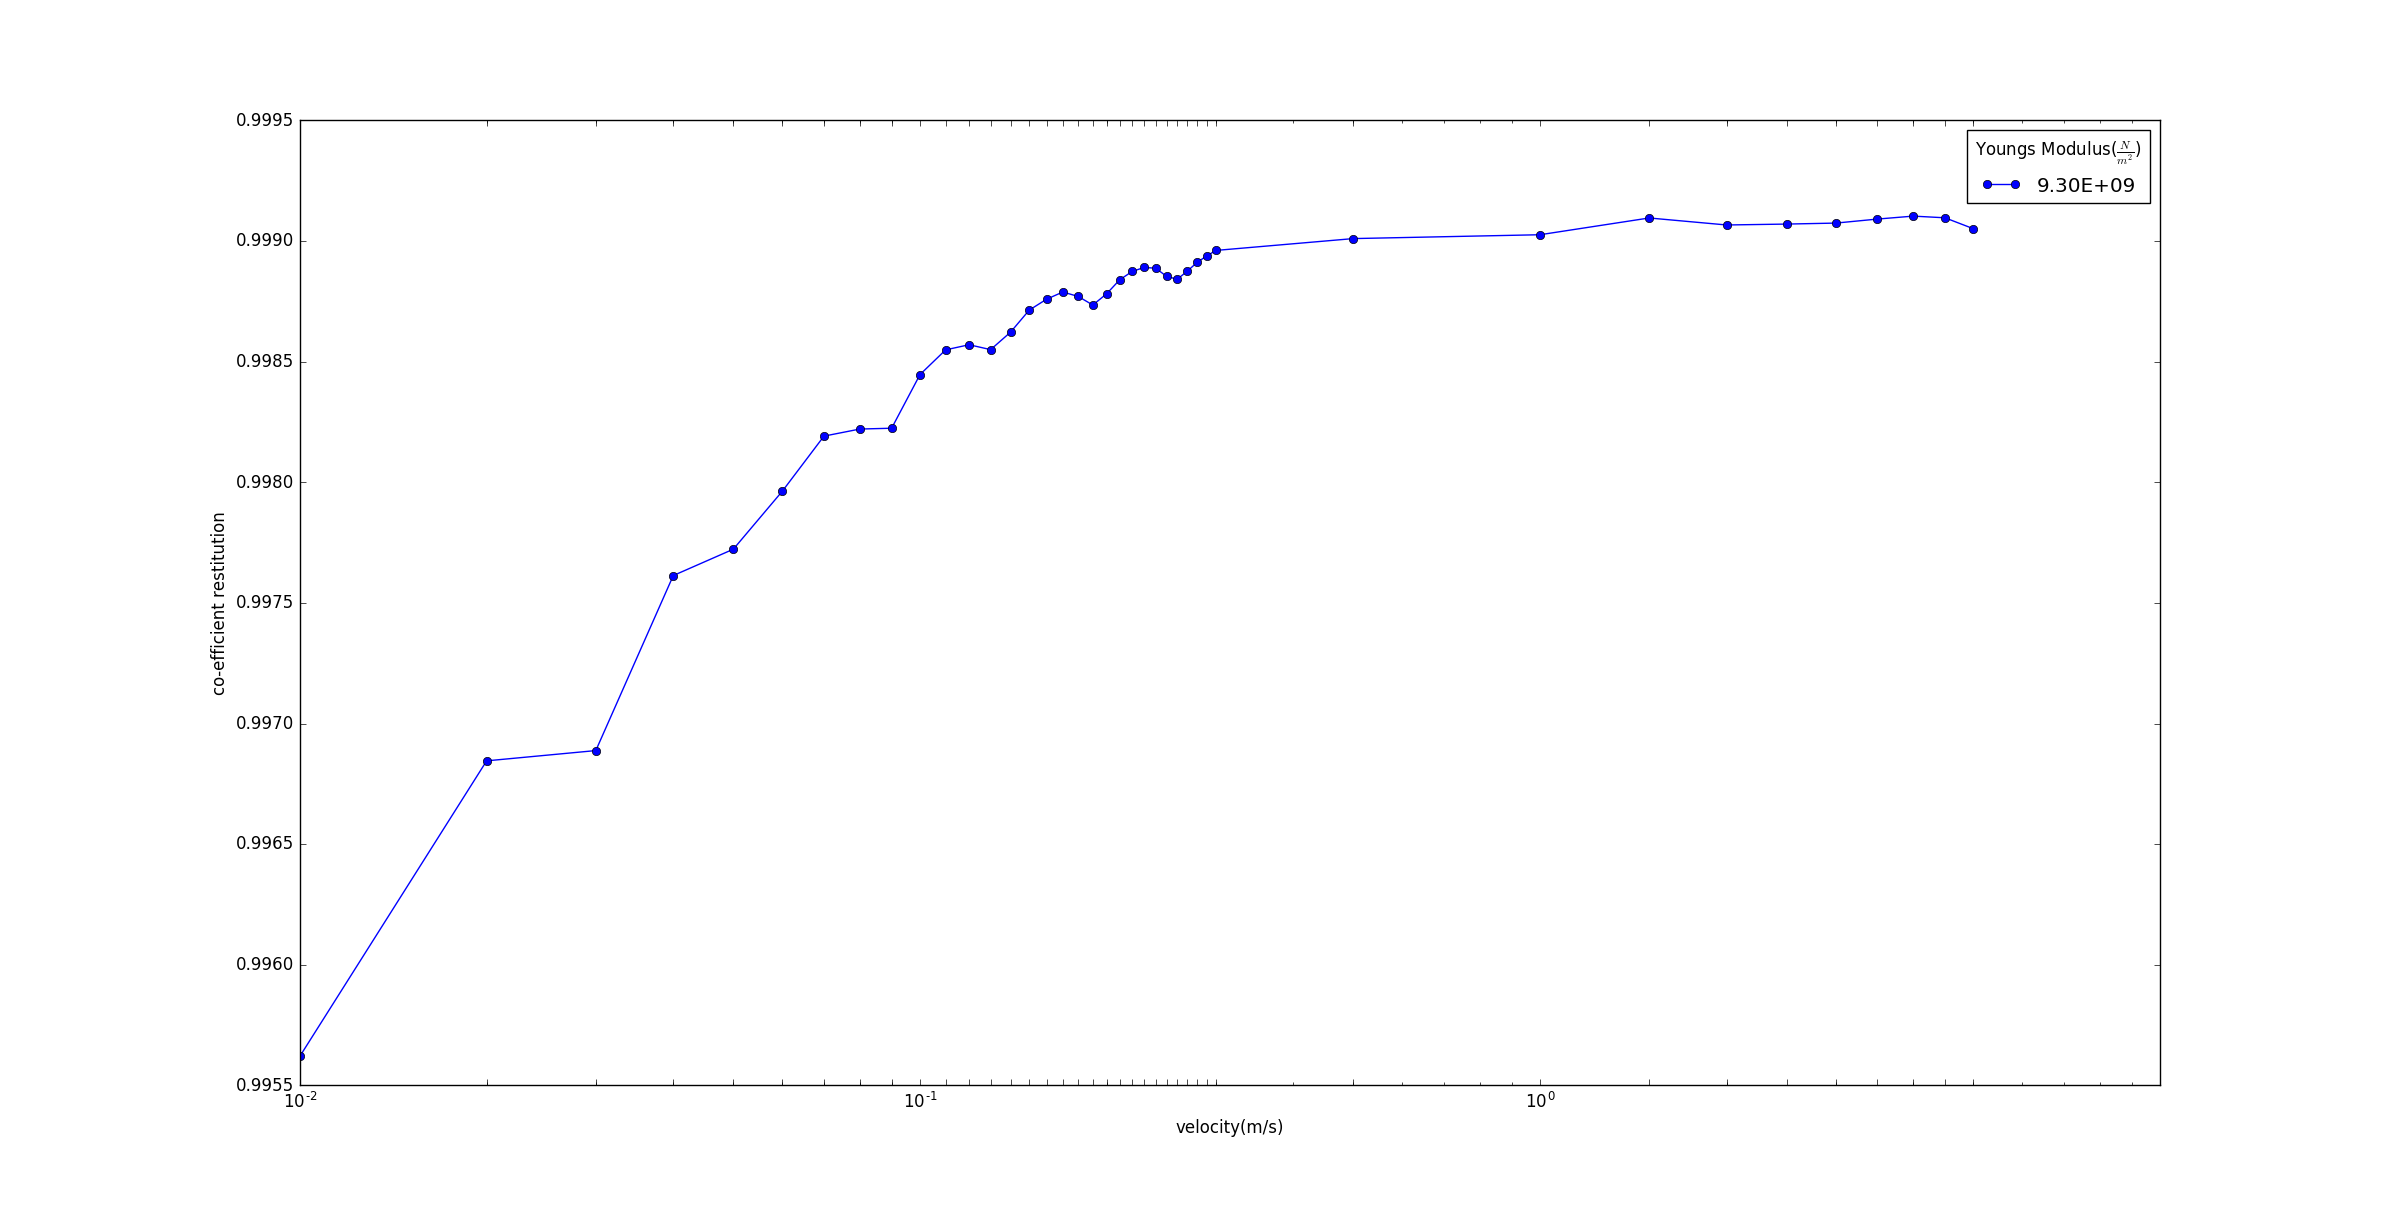
\includegraphics[width=1.0\textwidth]{../images/COR/COR.png}
\caption{Co-efficient of restitution}
\label{fig:COR}
\end{figure}

To understand the loss of energy to vibrations, the co-efficient of restitution was calculate for an elastic material with $Youngs Modulus(E)$ of $9.3GPa$ and various impact velocities ranging from $0.01m/s$ to $5m/s$.
The co-efficient of restitution was calculated by,
\begin{equation}
COR = \sqrt{\frac{Kinetic\, Energy\, after\, impact}{Kinetic\, Energy\, before\, impact}}
\end{equation}
Kinetic Energy was used to calculate the co-efficient of restitution because, calculating trajectory of the center of mass of the model was much more computationally intensive and inaccurate than calculate the Kinetic energy of the complete.
Measure the co-efficient of restitution is a measure of the restitution of kinetic energy after the collision of two objects. The figure \ref{fig:COR} shows the co-efficient of restitution vs various impact velocities. We can see that the co-efficient of restitution increases as the impact velocities are increased. The bumps in the plot can be explained after performing a Fourier analysis on the models. The Fourier analysis shows that the bumps correspond to the eigen modes of the model.

\subsection{Modal Analysis}


\begin{figure}[H]
\centering
\subfloat[Breathing Mode]{
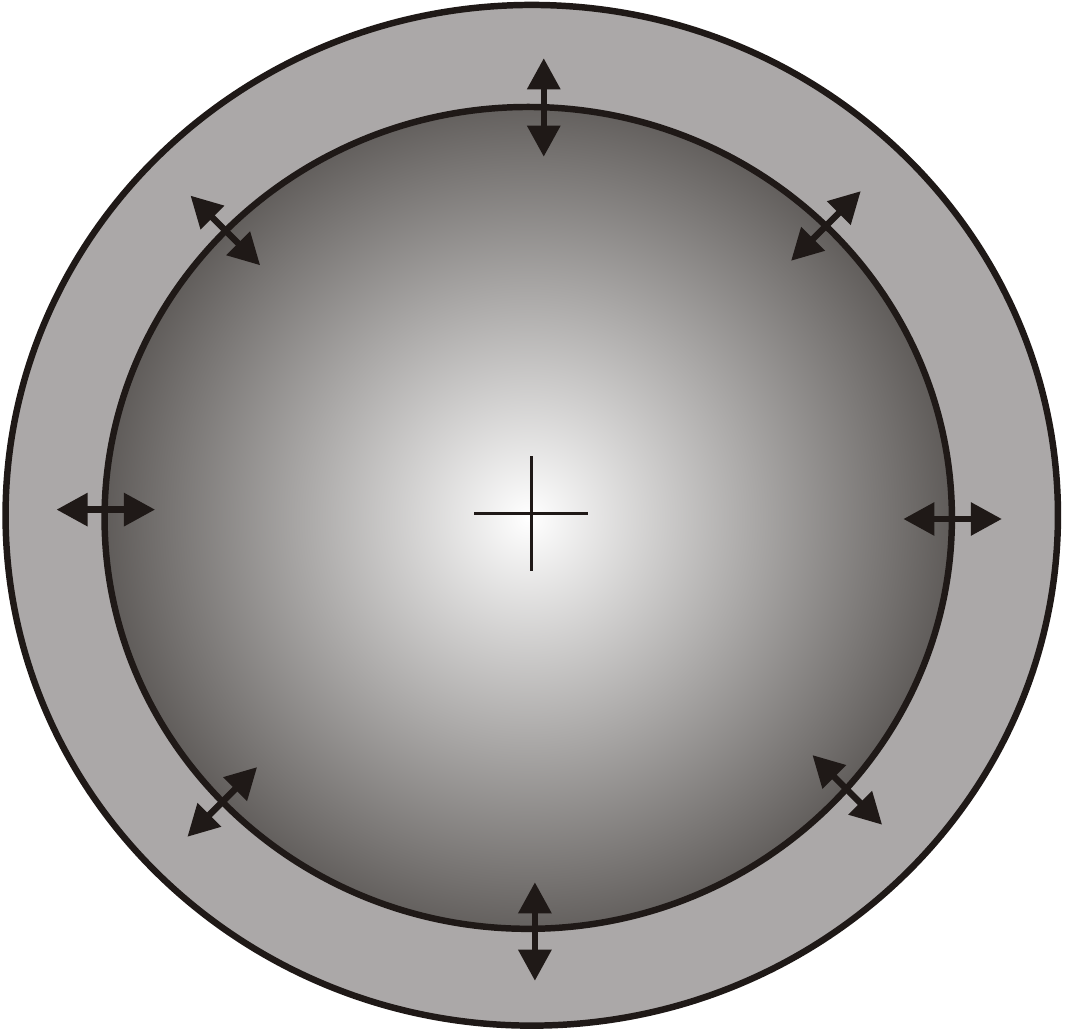
\includegraphics[width=0.45\textwidth]{../images/fft/breathinMode.png}
\label{fig:breath}
}
\subfloat[Prolate Oblique Mode]{
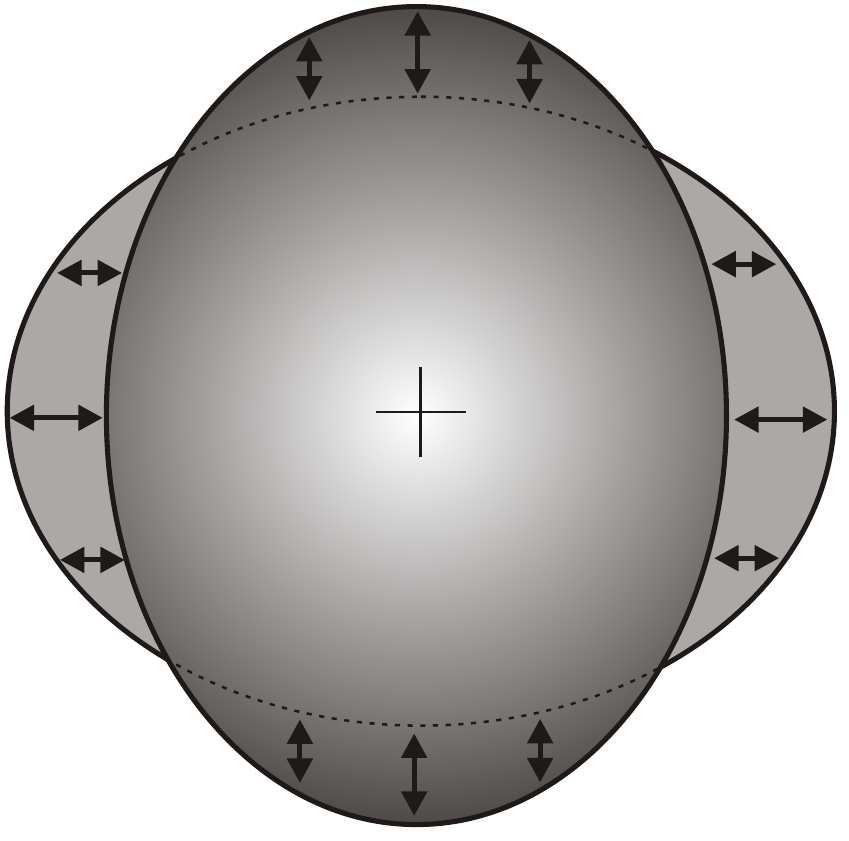
\includegraphics[width=0.45\textwidth]{../images/fft/prolateOblateMode.png}
\label{fig:prolate}
}
\caption{Different modes of vibration}
\label{fig:modes}
\end{figure}

To understand the plot \ref{fig:COR}, the modal analysis of the sphere was necessary. The natural frequencies of the sphere can affect the trajectory of the sphere during the impact. The two natural modes are shown in \ref{fig:modes}.

The modes shown in \ref{fig:modes} can affect the velocity of the sphere after the impact is complete. For example, when the sphere is in the prolate mode during towards the end of the impact, the velocity of the sphere increases as the direction of the sphere and the natural vibration modes are the same and decreases if the sphere is in the oblate mode during the end of the impact. 

\subsubsection{Eigen Frequencies of an elastic sphere}

\paragraph{Breathing Mode}

Using equation form the book "A Treatise on the Mathematical Theory of Elasticity" by A.E.H. Love, chapter 11:Vibration of spheres \citep{aelove}.

\begin{equation}
\begin{split}
\frac{h_{a}}{\pi} = 0.8160 = \frac{\frac{2R}{v_{dil}}}{T_{os}}\\
v_{dil} = \sqrt{\frac{\lambda + 2\mu}{\rho}}
\end{split}
\label{eq:eigen}
\end{equation} 
where $\frac{\pi}{h_{a}}$ is the ratio of the period of oscillation of the time taken by a wave of dilation to travel over a  distance equal to the diameter of the sphere, $v_{dil}$ is the velocity of the wave of dilation, $R$ is the radius of the sphere, $T_{os}$ is the time period of 1 oscillation, $\lambda and \mu$ are the lame's constants and $\rho$ is the mass density.

\begin{align}
T_{os} = \frac{1}{F} = \frac{2R}{v_{dil}} \frac{\pi}{h_{a}} = \frac{2R}{v_{dil}} \frac{1}{0.8160}
\end{align}

Poissons condition $\Rightarrow \lambda = \mu \Rightarrow \nu=\frac{1}{4}$

Therefore,
\begin{align}
 v_{dil} = \sqrt{\frac{3\lambda}{\rho}}
\end{align}

and since
\begin{align}
\lambda = \nu \ \frac{E}{2(1+\nu)} = \frac{E}{2(\frac{5}{4})} = \frac{2E}{5}
\end{align}

$v_{dil}$ now becomes
\begin{align}
v_{dil} = \sqrt{\frac{6E}{5\rho}}
\end{align}

we now have a equation for $T_{os}$
\begin{align}
T = 2R \sqrt{\frac{5\rho}{6E}} \frac{1}{0.8160}
\end{align}

For $R=0.01m, E=9.3Gpa$ and $\rho=900kg/m^{3}$
\begin{align}
T = 2\times 0.01 \sqrt{\frac{5 \times 900}{6 \times 9.3\times 10^{9}}} \frac{1}{0.8160} = 0.00000696031s \\
F = \frac{1}{T} = 143671.625591 Hz
\end{align} 


\paragraph{Prolate Oblate Mode}
Again using equation form the book "A Treatise on the Mathematical Theory of Elasticity" by A.E.H. Love, chapter 11:Vibration of spheres \citep{aelove}.

\begin{align}
\frac{\kappa_{a}}{\pi} = \frac{\frac{2R}{v_{dist}}}{T_{os}} = 1.8346
\end{align}
where $\frac{\pi}{\kappa_{a}}$ is the ratio of the period of oscillation to the time taken by a wave of distortion to travel over a distance equal to the diameter of the sphere and $v_{dist}$ is the velocity of the wave of distortion.

\begin{align}
v_{dist} = \sqrt{\frac{\mu}{\rho}} = \sqrt{\frac{2E}{5\rho}}
\end{align}

\begin{align}
T = \frac{2R}{\sqrt{\frac{2E}{5\rho}}\times 1.8346}
= 2R \sqrt{\frac{5\rho}{2E}} \frac{1}{1.8346}
\end{align}
For $R=0.01m, E=9.3Gpa$ and $\rho=900kg/m^{3}$

\begin{align}
T = 2\times 0.01 \sqrt{\frac{5*900}{2*9.3*10^9}} \frac{1}{1.8346} = 0.00000536214s
\end{align} 

\begin{align}
F = \frac{1}{T} = 186492.602141Hz
\end{align}

\begin{figure}[H]
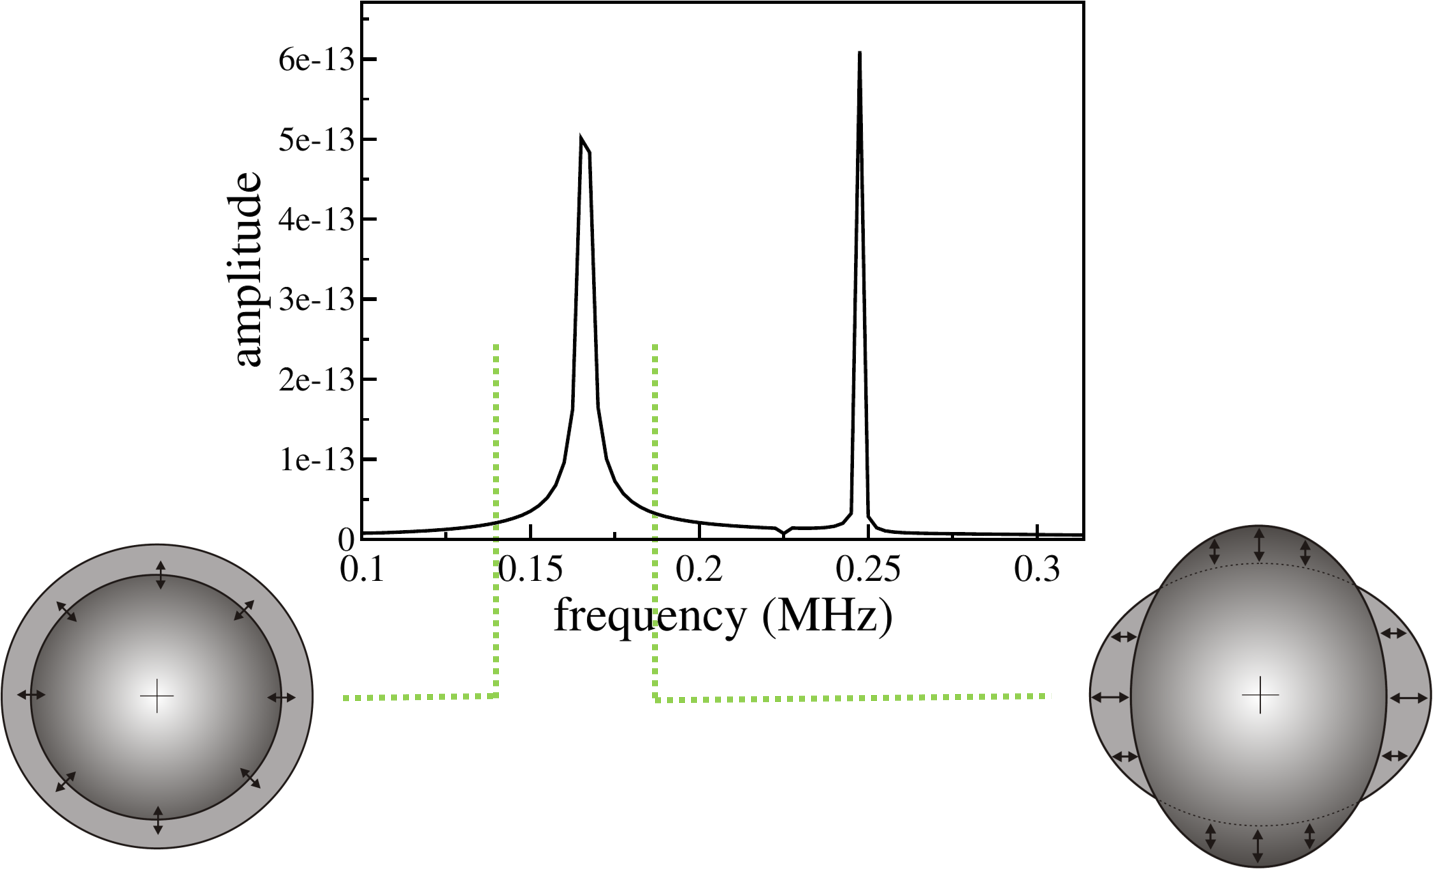
\includegraphics[scale=0.5]{../images/fft/spectrummodes.png}
\caption{Fourier Transform of Strain Energy}
\label{fig:spectrum}
\end{figure}

Now performing a fourier transform on the data of the strain energy remaining in the sphere after the impact is complete the frequency spectrum shown in \ref{fig:spectrum} was obtained.

\begin{figure}[H]
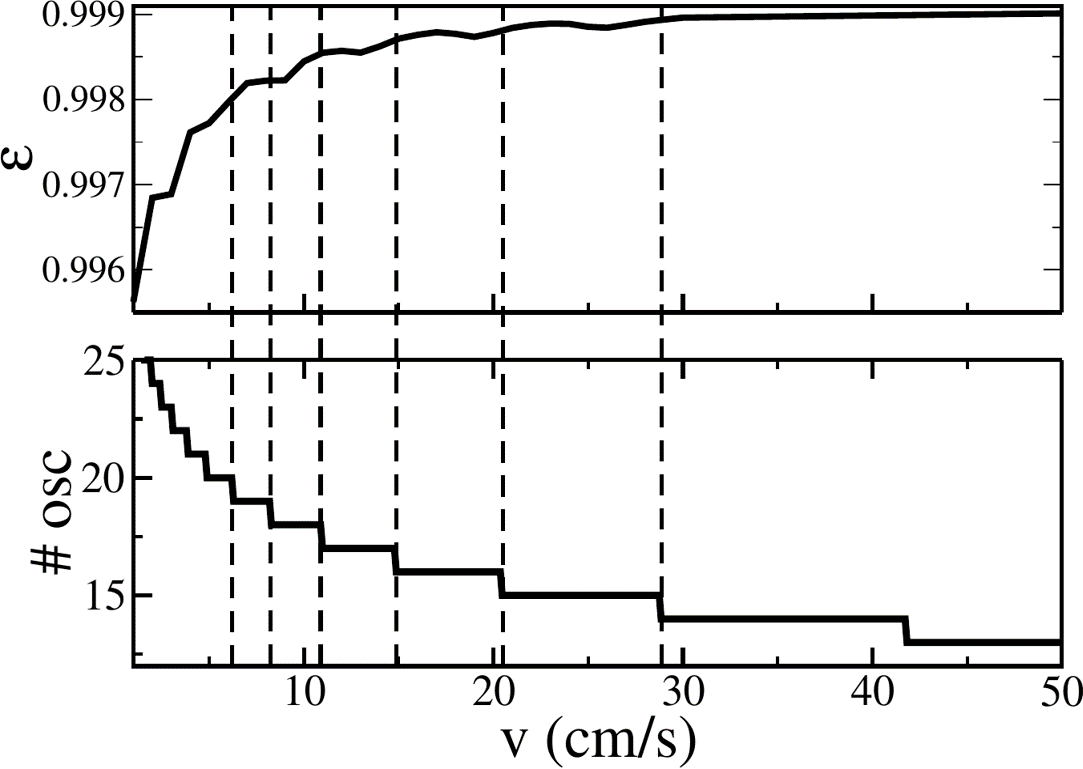
\includegraphics[scale=0.5]{../images/fft/oscillations.png}
\caption{Number of oscillation during contact}
\label{fig:oscillations}
\end{figure}

Now we calculate the number oscillations of the during the time of contact. When the plot of co-efficient of restitution and number of oscillation \ref{fig:oscillations} is compared, we observe whenever the number of completed oscillations increments by 1, the plot \ref{fig:COR} tends to dip and create a valley. This shows when the sphere is in the oblate  phase of the vibration, it results in a higher after impact velocity, hence create a bump in the plot of the co-efficient of restitution.




\section{Parametric Study}

%%%%%%%%%%%%%%%%%%%%%%%%%%%%%%%%%%%%%%%%%%%%
The next step of further study would be to experiment with various parameters such as material and diameter of the sphere.


\subsection{Different Youngs Modulus}

\begin{figure}[H]
\includegraphics[width=1.0\textwidth]{../images/parametricStudy/COR.png}
\caption{Co-efficient of restitution for various Youngs Modulus}
\label{fig:CORdiffEcomplete}
\end{figure}

The simulation was performed for a range of Youngs Modulii ranging from $1e8N/m^{2}$ to $1e11N/m^{2}$. It can be observed from the plots \ref{fig:CORdiffEcomplete}, for higher velocities as the $E$ increases the COR saturates to a level, which implies for materials for higher $E$, the percentage loss of kinetic energy remain constant. Whereas for lower velocities we see the reverse plots, i.e higher $E$'s have a lower co-efficient of restitution. This results was unexpected as the expected result was a gradual increase in co-efficient of restitution as the $E$ increases. 

%%%%%%%%%%%%%%%%%%%%%%%%%%%%%%%%%%%%%%%%%%%%

\subsection{Different Diameters}

\begin{figure}[H]
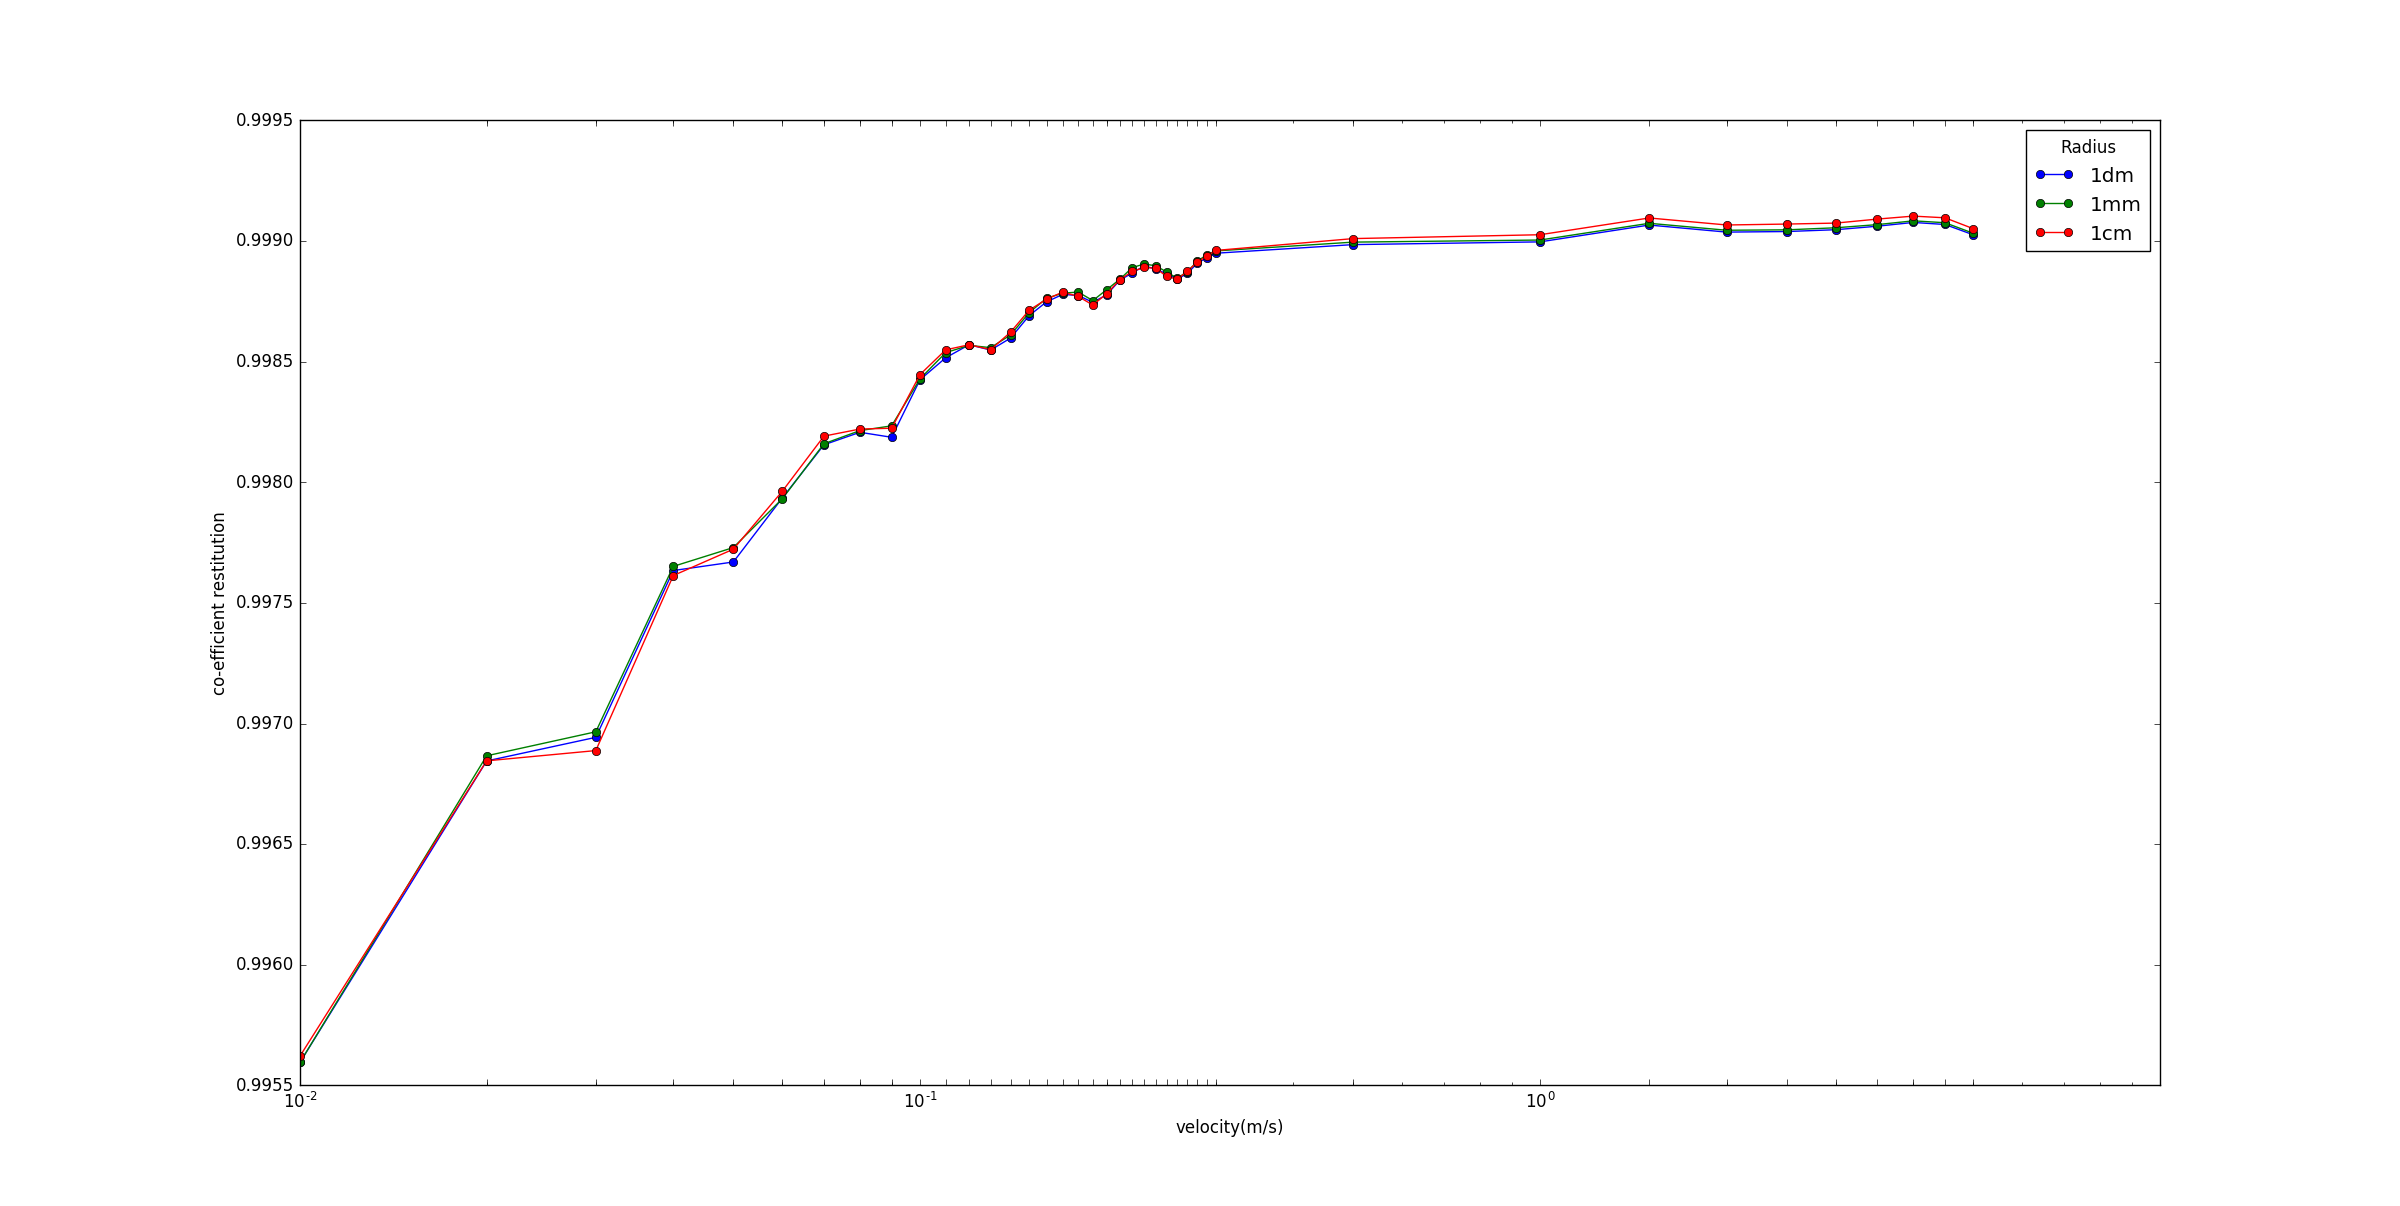
\includegraphics[width=1.0\textwidth]{../images/parametricStudy/CORvsVELdiffDAI.png}
\caption{Co-efficient of restitution for various radii}
\label{fig:CORDiffDia}
\end{figure}

The simulation was also performed for various spheres of diameters of $0.001m$, $0.01m$ and $0.1m$. Considering the equations for coefficient of restitution from \citep{muller} .

\begin{align*}
\varepsilon = 1+ \sum_{k=0}^{\infty} h_{k}(\beta^{\frac{1}{2}} v^{\frac{1}{10}})^{k} 
\end{align*}

where
\begin{align*}
\beta &= \frac{3}{2} A (\frac{\rho}{m_{eff}})^{\frac{2}{5}} \\
\beta &\propto (\frac{\rho}{m_{eff}})^{\frac{2}{5}}
\end{align*}

also 
\begin{align*}
\rho \propto \sqrt{R}, \quad m_{eff} \propto R^{3}
\end{align*}

therefore

\begin{align*}
\beta \propto \Big( \frac{\sqrt{R}}{R^{3}} \Big)^{\frac{2}{5}} = R^{-1}
\end{align*}

Hence we see, for a viscoelastic case the co-efficient of restitution is inversely proportional to the radius. A similar result was expected for the elastic case, but the plot \ref{fig:CORDiffDia} does not agree. We see there is no effect of diameter on the co-efficient of restitution in the elastic case.
%%%%%%%%%%%%%%%%%%%%%%%%%%%%%%%%%%%%%%%%%%%%



